\documentclass[11pt,a4paper]{article}
\usepackage[hyperref]{acl2018}
\usepackage{times}
\usepackage{latexsym}

\usepackage[letterpaper]{geometry}
%\usepackage{amta2016}
\usepackage{url}
\usepackage{natbib}
\usepackage{layout}
\usepackage{algorithmic}
\usepackage{algorithm}
\usepackage{graphicx}
\usepackage{amsmath}
\DeclareMathOperator*{\argmax}{argmax}

\newcommand{\confname}{AMTA 2016}
\newcommand{\website}{\protect\url{http://www.amtaweb.org/}}
\newcommand{\contactname}{research track co-chair Lane Schwartz}
\newcommand{\contactemail}{lanes@illinois.edu} 
\newcommand{\conffilename}{amta2016}
\newcommand{\downloadsite}{\protect\url{http://www.amtaweb.org/}}
\newcommand{\paperlength}{$12$ (twelve)}
\newcommand{\shortpaperlength}{$6$ (six)}

%% do not add any other page- or text-size instruction here

\parskip=0.00in

\begin{document}

% \mtsummitHeader{x}{x}{xxx-xxx}{2016}{45-character paper description goes here}{Author(s) initials and last name go here}
\title{\bf Faster Neural Machine Translation Inference}  

\author{\name{\bf Hieu Hoang} \hfill  \addr{hieu@hoang.co.uk}\\ 
        \addr{}
\AND
       \name{\bf Tomasz Dwojak} \hfill \addr{???}\\
        \addr{Adam Mickiewicz University}
\AND
       \name{\bf Kenneth Heafield} \hfill \addr{???}\\
       %\name{\bf Kenneth Heafield} \hfill \addr{kheafiel@inf.ed.ac.uk}\\
        \addr{University of Edinburgh, Scotland}
}

\maketitle
\pagestyle{empty}

\begin{abstract}

Deep learning models are widely deployed for machine translation. In comparison on many other deep learning models, there are two characterisitics of machine translation which have not been adequately addressed by most software implementations, leading to slow inference speed. Firstly, as opposed to standard binary class models, machine translation models are used to discriminate between a large number of classes corresponding to the output vocabulary. Secondly, rather than a single label, the output from machine translation models is a sequence of class labels that makes up the words in the target sentence. The sentence lengths are unpredictable, leading to inefficiencies during batch processing. We provide solutions for these issues which together, increase batched inference speed by up to ??? on modern GPUs without affecting model quality. For applications where the use of maxi-batching introduces unacceptable delays in response time, our work speed up inference speed by up to ???. Our work is applicable to other language generation tasks and beyond.

\end{abstract}

\section{Introduction}

We will look at two areas that are critical to fast NMT inference where the models in NMT differ significantly from those in other applications. These areas have been overlooked by the general deep-learning community, we aim to improve their efficient for NMT-specific tasks.

Firstly, the number of classes in many deep-learning applications is small. However, the number of classes in NMT models is typically in the tens or hundreds of thousands, corresponding to the vocabulary size of the output language. For example, ~\cite{sennrich-haddow-birch:2016:P16-12} experimented with target vocabulary sizes of 60,000 and 90,000 subword units. This makes the output layer of NMT models very computationally expensive. Figure~\ref{fig:pie-time} shows the breakdown of amount of time during translation our NMT system; nearly 70\% of the time is involved in the output layer. We will look at optimizations which explicitly target the output layer.
\begin{figure}
\centering
\begin{tabular}{cc}
{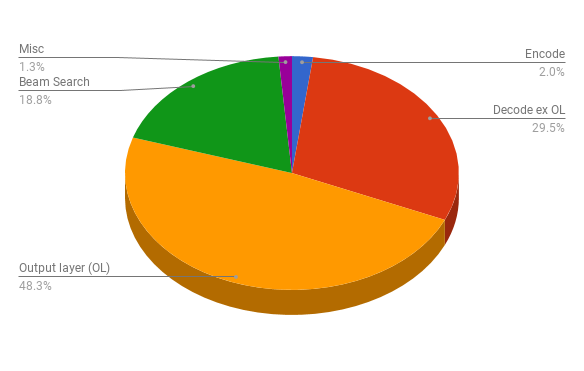
\includegraphics[scale=0.3]{pie-time-europarl.png}} 
\end{tabular}
\caption{Time spent during translation (beam size 5, Europarl test set)}
\label{fig:pie-time}
\end{figure} 

Secondly, the use of mini-batching is critical for fast model inference. However, mini-batching does not take into acccount variable sentence lengths which decrease the actual number of input or output sentences that are processed in parallel, negating the benefit of mini-batching. This can be partially reduced in the encoding with \emph{maxi-batching}, i.e. pre-sorting sentences by length before creating mini-batches with similar length source sentences. However, target sentence lengths will still differ even for similar length inputs, compromising decoding performance. Figure~\ref{fig:batch-size} shows the actual batch size during decoding with a maximum batch size of 128; in only 42\% of decoding iteration was batch full.

\begin{figure}
\centering
\begin{tabular}{cc}
{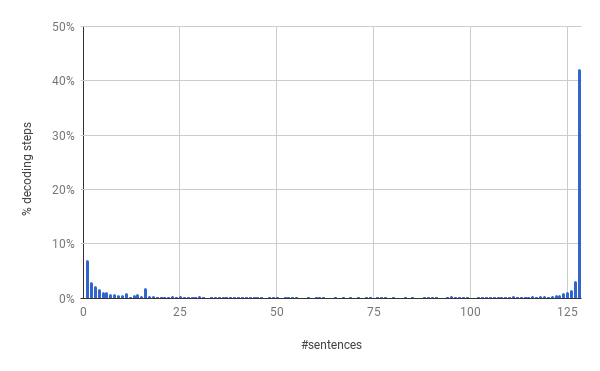
\includegraphics[scale=0.3]{batch-size.png}} 
\end{tabular}
\caption{Actual batchsize during decoding (max batchsize 128, beam size 5, Europarl test set)}
\label{fig:batch-size}
\end{figure} 

We will propose an alternative batching algorithm to increase the actual batch size during decoding.

We base our model on the sequence-to-sequence model of ~\cite{D14-1179} for machine translation models and also choose to focus on the using GPUs rather than CPUs as pursued by ~\cite{DBLP:conf/emnlp/Devlin17}.

\section{Prior Work}

Deep learning models have been successfully used on many machine learning task in recent years in areas as diverse as computer vision and natural language processing. This success have been followed by the rush to put these model into production. However, the computational resources required in order to run these models have ben chanllenging. One possible solution involves creating faster models that can approximate the original model~\citep{DBLP:conf/emnlp/KimR16}. Another solution is tackling specific computationally intensive functions by approximating them (??? softmax). 

Most current neural MT models follow an encoder-decoder architecture. The encoder calculates the word and sentence embeddings while the decoder generates the output sentence. The architecture within the encoder is still a subject of much research. ~\cite{kalchbrenner13emnlp} used a convolution to encode the input and a recurrent neural network (RNN) for the decoder. RNNs was used for both encoding and decoding in (??? who used RNN 1st). ~\cite{Sutskever:2014:SSL:2969033.2969173} significantly improved translation quality by using LSTM was used in each RNN node. ~\cite{D14-1179} used GRU that has the required properties of LSTM but is computationally cheaper. ~\cite{DBLP:journals/corr/BahdanauCB14} added attention model which improved translation at a cost of slower speed.

There has been recent attempts to move away from the sequence-to-sequence models of RNN encoder-decoder. Some justify their architecture on faster inference as well as better translation results. ~\cite{DBLP:journals/corr/VaswaniSPUJGKP17} and (??? course-to-fine) has been proposed as a fast alternatives to RNN-based models as it is possible to process more of the units in parallel.

It has been noticed that half precision arithmetic can be used for deep learning model without significan loss of model quality~\citep{DBLP:journals/corr/abs-1710-03740}. Other solutions include specialized hardware, the most popular being graphical processing units (GPU) but other hardware such as custom processors TPU~\citep{DBLP:journals/corr/JouppiYPPABBBBB17}, FPGA~\citep{DBLP:journals/corr/LaceyTA16} have been used. 

Many of these optimization are general purpose improvements for deep learning models, regardless of the task it is being used in. ~\cite{DBLP:conf/emnlp/Devlin17} is a noticeable machhine translation-specific optimization which describe the speed improvements that can be obtained by techniques such as the use of half-precision, model changes and pre-computation.

\section{Proposal}
\label{sec:Proposal}

\subsection{Softmax and Beam Search Fusion}

The output layer of most deep learning models consist of the following steps
\begin{enumerate}
   \item \vspace{-2 mm} multiplication of the input with the weight matrix $p = w x$
   \item \vspace{-2 mm} addition of a bias term to the resulting scores $p = p + b$
   \item \vspace{-2 mm} applying the activation function, most commonly softmax $ p_i = \exp(p_i) / \sum \exp(p_i) $
   \item \vspace{-2 mm} a search for the best output class, and probability if necessary $\argmax_i p_i$
\end{enumerate}

In models with a small number of classes such as binary classification, the computational effort required is trivial and fast. However, this is not the case for large number of classes such as those found in NMT models.

We shall leave step 1 for future work and focus on the last three steps, the outline for which are shown in Figures~\ref{algo:Add Bias Term} to ~\ref{algo:Find best}.

\begin{figure} [h]
\begin{algorithmic}
\REQUIRE vector $p$, bias vector $b$
\FORALL{$p_i$ in $p$}
  \STATE $p_i \gets p_i + b_i$
\ENDFOR 
\end{algorithmic}
\caption{Add Bias Term}
\label{algo:Add Bias Term}
\end{figure}

\begin{figure} [h]
\begin{algorithmic}
\REQUIRE vector $p$

\COMMENT{calculate max for softmax stability}

\STATE $max \gets - \infty$ 
\FORALL{$p_i$ in $p$}
  \IF{$p_i > max$}
    \STATE $max \gets p_i$
  \ENDIF
\ENDFOR 

\COMMENT{calculate denominator}

\STATE $sum \gets 0$ 
\FORALL{$p_i$ in $p$}
  \STATE $sum \gets sum + \exp(p_i - max)$
\ENDFOR 

\COMMENT{calculate softmax}

\FORALL{$p_i$ in $p$}
  \STATE $p_i \gets \frac{\exp(p_i) - max}{sum} $
\ENDFOR 

\RETURN $p$

\end{algorithmic}
\caption{Calculate softmax}
\label{algo:Calculate softmax}
\end{figure}

\begin{figure} [h]
\begin{algorithmic}
\REQUIRE softmax vector $p$

\STATE $max \gets - \infty$ 
\FORALL{$p_i$ in $p$}
  \IF{$p_i > max$}
    \STATE $max \gets p_i$
    \STATE $best \gets i$
  \ENDIF
\ENDFOR 

\RETURN $max$, $best$

\end{algorithmic}
\caption{Find best}
\label{algo:Find best}
\end{figure}


As can be seen, the operations iterate over the matrix p five times - once to add the bias, three times to calculate the softmax, and once to search for the best class. We shall use a popular method, kernel fusion~\citep{Guevara2009EnablingTP}, to optimize the output layer.

Secondly, we make use of the fact that softmax and $\exp$ are monotonic functions therefore we can move the search for the best class from Figure~\ref{algo:Find best} to Figure~\ref{algo:Calculate softmax} while $max$ is being sought.

Thirdly, we are only interested in the best class. Since the best class is known, we can avoid calculating softmax for all classes. The outline of the our function is shown in Figure~\ref{algo:Fused Kernel}.

\begin{figure} [h]
\begin{algorithmic}
\REQUIRE vector $p$, bias vector $b$

\COMMENT{add bias, calculate $max$ \& $argmax$}

\STATE $max \gets - \infty$ 
\FORALL{$p_i$ in $p$}
  \IF{$p_i + b_i > max$}
    \STATE $max \gets p_i + b_i$
    \STATE $best \gets i$
  \ENDIF
\ENDFOR 

\COMMENT{calculate denominator}

\STATE $sum \gets 0$ 
\FORALL{$p_i$ in $p$}
  \IF{$p_i > max$}
    \STATE $sum \gets sum + \exp(p_i - max)$
  \ENDIF
\ENDFOR 

\RETURN $\frac{1}{sum}$, $best$ 


\end{algorithmic}
\caption{Fused softmax and argmax}
\label{algo:Fused Kernel}
\end{figure}


In fact, we are usually only interested in the best class during inference, not the probability. Therefore, we can skip the second iteration over $p$ in Figure~\ref{algo:Fused Kernel} and avoid computing the softmax altogether. %, Figure~\ref{algo:Argmax only}.

% \begin{figure} [h]
% \begin{algorithmic}
% \REQUIRE activation vector $p$, bias vector $b$
% 
% \COMMENT{add bias, calculate $argmax$}t
% \FORALL{$p_i$ in $p$}
%   \IF{$p_i + b_i > max$}
%     \STATE $max \gets p_i + b_i$
%     \STATE $argmax \gets i$
%   \ENDIF
% \ENDFOR 
% 
% 
% \RETURN $argmax$ 
% 
% \end{algorithmic}
% \caption{Argmax only}
% \label{algo:Argmax only}
% \end{figure}

It has been shown ~\citep{koehn-knowles:2017:NMT} that using beam search to use the n-best number of classes, rather than just the best class, improves translation quality. This is a simple extension to the algorithm of Figure~\ref{algo:Fused Kernel}. Unlike the 1-best case, however, the softmax calculation cannot be skipped as the denominator differs for each input.


\subsection{Top-up Batching}

The standard mini-batching algorithm is outlined in Figure~\ref{algo:Mini-batching}.

\begin{figure} [h]
\begin{algorithmic}
%\REQUIRE source sentence $s$, translation options
\WHILE{more input} 
  \STATE Create batch
  \STATE Encode
  \WHILE{batch is not empty} 
    \STATE Decode batch
    \FOR{each sentence in batch}
      \IF{translation is complete}
        \STATE Remove sentence from batch
      \ENDIF
    \ENDFOR
  \ENDWHILE
\ENDWHILE 
\end{algorithmic}
\caption{Mini-batching}
\label{algo:Mini-batching}
\end{figure}

This algorithm encode the sentences for a batch, followed by decoding the batch. The decoding stop once all sentences in the batch are completed. This is a potential inefficiency as the number of remaining sentences may not be optimal.

We will focus on decoding as this is the more compute-intensive step, and issues with differing sentence sizes in encoding can partly be ameriorated by maxi-batching.

Our proposed top-up batching algorithm encode and decode asynchronously. The encoding step, Figure~\ref{algo:Encoding for top-up batching}, is similar to the main loop of the standard algorithm but the results are added to a queue to be consumed by the decoding step later.

\begin{figure} [h]
\begin{algorithmic}
%\REQUIRE source sentence $s$, translation options
\WHILE{more input} 
  \STATE Create encoding batch
  \STATE Encode
  \STATE Add to queue
\ENDWHILE 
\end{algorithmic}
\caption{Encoding for top-up batching}
\label{algo:Encoding for top-up batching}
\end{figure}

Rather than decoding the same batch until all sentences in the batch are completed, the decoding step processing the same batch continuously. New sentences are added to the batch as old sentences completes, Figure~\ref{algo:Decoding for top-up batching}.

\begin{figure} [h]
\begin{algorithmic}
%\REQUIRE source sentence $s$, translation options
\STATE create decoding batch $b$ from queue
\WHILE{$b$ is not empty}
  \STATE Decode $b$
  \STATE Replace completed sentences with new sentence from queue
\ENDWHILE 
\end{algorithmic}
\caption{Decoding for top-up batching}
\label{algo:Decoding for top-up batching}
\end{figure}


\section{Experimental Setup}
\label{sec:Experimental Setup}

We trained a sequence-to-sequence, encoder-decoder NMT system similar to that described in ~\cite{sennrich-haddow-birch:2016:P16-12}. This uses recurrent neural networks with gated recurrent units. The input and output vocabulary size were both set to 85,000 subwords using byte-pair encoding (BPE) to adjust the vocabulary to the desired size. The hidden layer dimensions was set to 512. %We used the Marian toolkit to train our models.

For inference, we used and extend Amun~\citep{junczys2016neural}, the fastest open-source inference engine we are aware of for the model used in this paper. We uused a mini-batch of 128 sentences and maxi-batch of 1280 sentences, unless otherwise stated.

The hardware used in all experiments was an Nvidia GTX 1060 GPU on a host containing 8 Intel hypercores running at 2.8Ghz, 16GB RAM and SSD hard drive.

Our training data consisted of the German-English parallel sentences from the Europarl corpus~\citep{Koehn:2005:MTS}. To test inference speed, we used two test sets with differing characteristics:
\begin{enumerate}
   \item \vspace{-2 mm} a subset of the Europarl training data, which contains mostly long sentences, and is, of course, in the same domain as the training data
   \item \vspace{-2 mm} a subset of the German-English data from the Open-Subtitles corpus, consisting of mostly short, out-of-domain sentences.
\end{enumerate}
Table~\ref{tab:corpora} gives further details of the test sets.

\begin{table}
\begin{center}
\small
\begin{tabular}{|l|r|r|} \hline
		  & Europarl		& OpenSubtitles \\ \hline
\# sentences  	  & 30,000 		& 50,000 \\
\# subwords 	  & 787,908 		& 467,654 \\ 
Avg subwords/sent & 26.3		& 9.4 \\ \hline
\end{tabular}
\end{center}
\caption{Test sets}
\label{tab:corpora}
\end{table}


\section{Results}
\label{sec:Results}

\subsection{Softmax and Beam Search Fusion}

Fusing the softmax and beam search increase the speed of the output layer by 43\% for beam size 1, decreasing to 25\% for a beam of 10 when translating the Europarl dataset. This led to an overall increase in translation speed of up to 23\%, Figure~\ref{fig:beam-europarl}. Translation speed improved by up to 41\% when translating the Opensubtitles datset, Figure~\ref{fig:beam-opensubtitles}. The amount of time taken to calculate the output layer dominates trannslation time for the short OpenSubtitles test set, Figure~\ref{fig:pie-time-opensubtitles}.

\begin{figure}
\centering
\begin{tabular}{cc}
{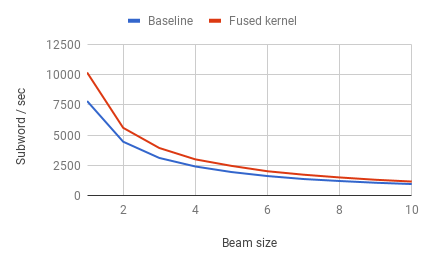
\includegraphics[scale=0.5]{beam-europarl.png}} 
\end{tabular}
\caption{Translation speed for Europarl test set}
\label{fig:beam-europarl}
\end{figure} 

\begin{figure}
\centering
\begin{tabular}{cc}
{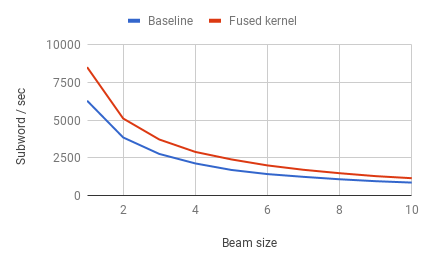
\includegraphics[scale=0.5]{beam-opensubtitles.png}} 
\end{tabular}
\caption{Translation speed for Opensubtitles test set}
\label{fig:beam-opensubtitles}
\end{figure} 

\begin{figure}
\centering
\begin{tabular}{cc}
{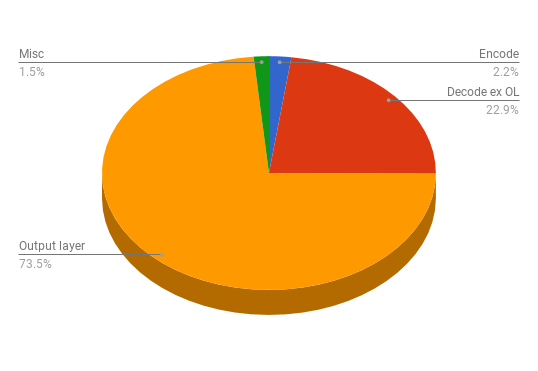
\includegraphics[scale=0.3]{pie-time-opensubtitles.png}} 
\end{tabular}
\caption{Time spent during translation (beam size 5, Opensubtitles test set)}
\label{fig:pie-time-opensubtitles}
\end{figure} 

\subsection{Top-up Batching}

\section{Conclusion}



%\section*{Acknowledgments}
%This work is sponsored by the Air Force Research Laboratory, prime contract FA8650-11-C-6160.  The views and conclusions contained in this document are those of the authors and should not be interpreted as representative of the official policies, either expressed or implied, of the Air Force Research Laboratory or the U.S. Government.

\bibliographystyle{apalike}
\bibliography{amta2016,mt,more}


\end{document}
\grid
